\tikzset{main node/.style={circle,fill=white!20,draw,minimum size=0.5cm,inner sep=0pt},}
\usetikzlibrary{graphs,graphs.standard}

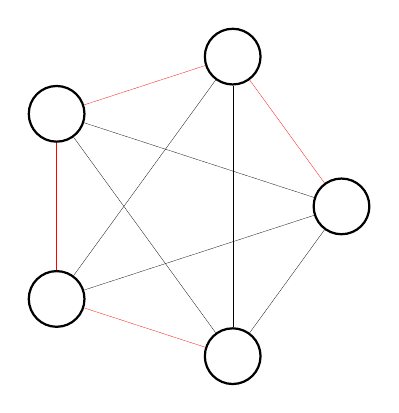
\begin{tikzpicture}
  \foreach \x in {1,...,5}{%
    \pgfmathparse{(\x-1)*360/5}
    \node[draw,circle,inner sep=0.25cm] (N-\x) at (\pgfmathresult:2.0cm) [thick] {};
  }
  \pgfmathparse{7*360/5}
  %\node[circle,red] (N-8) at (\pgfmathresult:5.4cm) {\ldots};
  
  \path (N-1) edge[ultra thin,-, red] (N-2);
  \path (N-2) edge[ultra thin,-, red] (N-3);
  \path (N-3) edge[ultra thin,-, red] (N-4);
  \path (N-4) edge[ultra thin,-, red] (N-5);
  
  \path (N-1) edge[ultra thin,-] (N-3);
  \path (N-1) edge[ultra thin,-] (N-4);
  \path (N-1) edge[ultra thin,-] (N-5);
  
  \path (N-2) edge[ultra thin,-] (N-4);
  \path (N-2) edge[ultra thin,-] (N-5);
  
  \path (N-3) edge[ultra thin,-] (N-5);
  
\end{tikzpicture}